\documentclass[a4 paper]{article}
\usepackage{amssymb,amsmath,graphicx,float,color, geometry}
\geometry{top=1in, bottom=1in}

%opening
\title{Investigating Drug Usage Patterns in the U.S.}
\author{Colin Van Oort}

\begin{document}

\maketitle

\begin{abstract}
It is estimated that the U.S. loses upwards of 700 billion dollars annually from crimes, health care costs, and lost productivity related to drug use \cite{NIDA}. In 2013 alone, 1.5 million people were arrested on non-violent drug charges and more than 40,000 people died from drug overdoses \cite{DPA}, thus it is of great financial and societal importance to investigate drug usage behavior. Using information provided by a sample population and a multitude of statistical and mathematical methods it is possible to tease out many patterns and correlations that exist in drug usage behavior. Important features which are investigated include which drugs are most used, when drug use usually begins, which drugs are most addictive, and more.
\end{abstract}


\section*{Data \& Methods}

The data set used in the creation of this report was provided by the United States Department of Health and Human Services as a part of the National Survey on Drug Use and Health in 2012 \cite{USDOH}. It was obtained in a tab separated value format and contains 3120 columns (survey answers / computed statistics) and 55268 rows (participants in the survey). No alterations were performed on the original data, since it was obtained in a structured format and came with detailed documentation it was used in its default state. The data was then manipulated and analyzed using the programming language python and the third party libraries matplotlib, scipy, and numpy which were used for implementations of plotting utilities and statistical methods.


\section*{Results}

\subsection*{Demographics}
Since the data was obtained by an external source it is important to inspect the demographics of the survey population in order to identify if it contains any biases, thus the gender, age, and race distributions of the sample populations are presented. 

\begin{figure}[H]
	\centering
	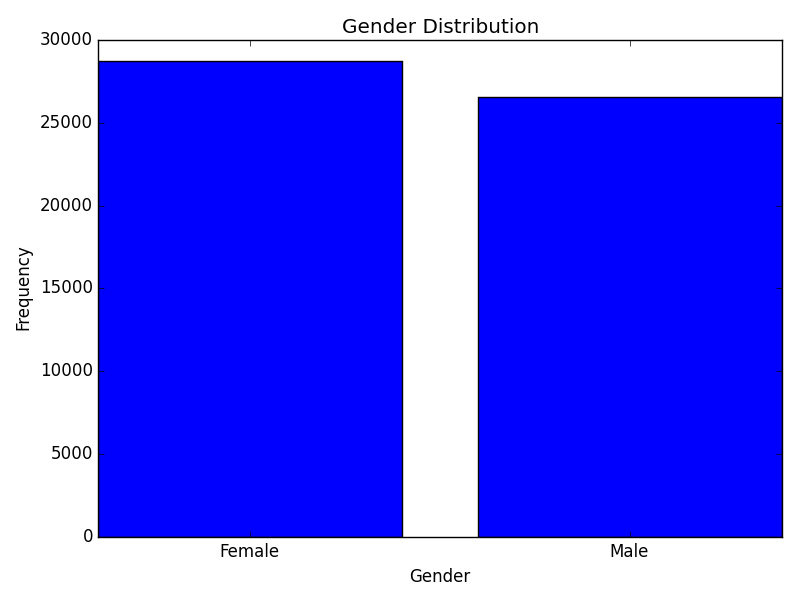
\includegraphics[width=5in]{images/genderDist}
	\caption{The gender distribution of the survey population}
\end{figure}

\begin{figure}[H]
	\centering
	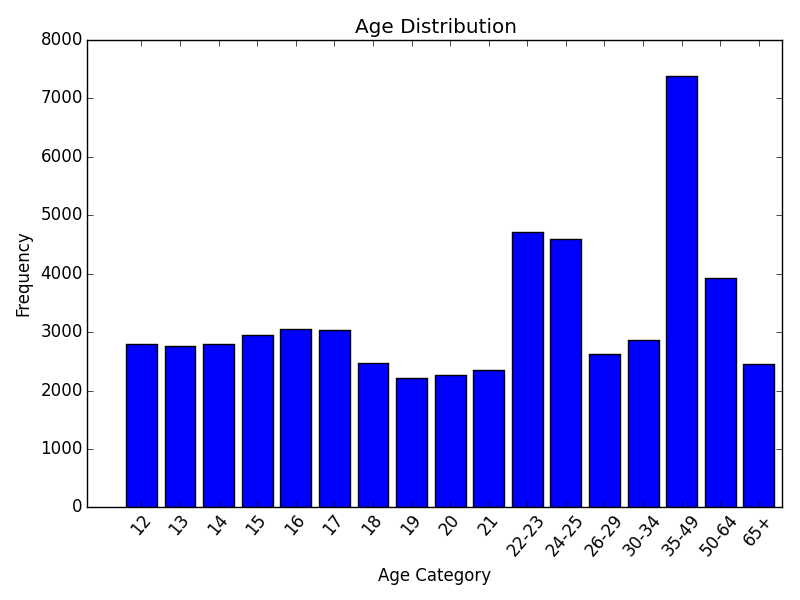
\includegraphics[width=5in]{images/ageDist}
	\caption{The age distribution of the survey population}
\end{figure}

\begin{figure}[H]
	\centering
	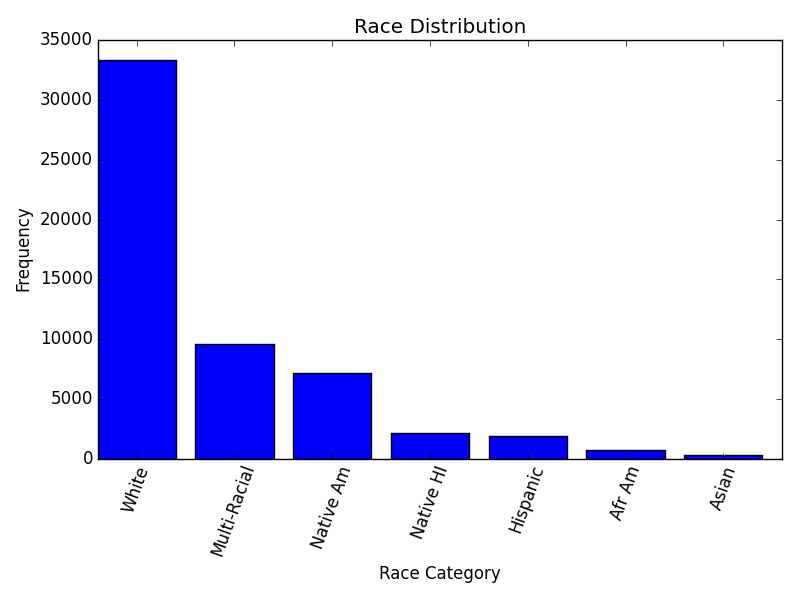
\includegraphics[width=5in]{images/raceDist}
	\caption{The racial distribution of the survey population}
\end{figure}

Figure 1 shows the population consists of roughly equal amounts of male and female participants, while Figure 2 and Figure 3 reveal a prevalence of middle aged (35-50) and college aged (22-25) participants as well as an overwhelming majority of the survey population identifying as white. \\


\subsection*{Alcohol \& Cigarettes}
Next the age of first use of alcohol and cigarettes are investigated due to their unique level of prevalence and acceptance in modern culture compared to the other drugs that the survey gathered information on.

\begin{figure}[H]
	\centering
	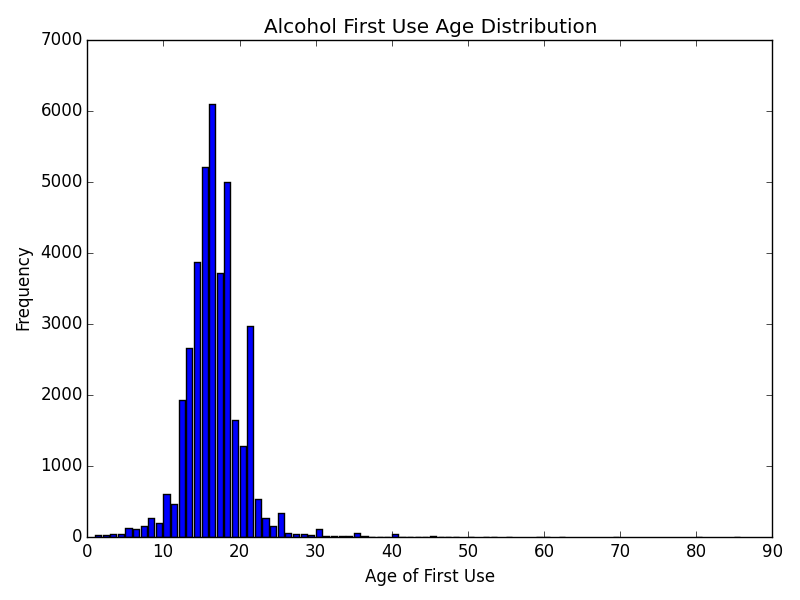
\includegraphics[width=5in]{images/alcAFU}
	\caption{Age of first use with regards to alcohol}
\end{figure}

\begin{figure}[H]
	\centering
	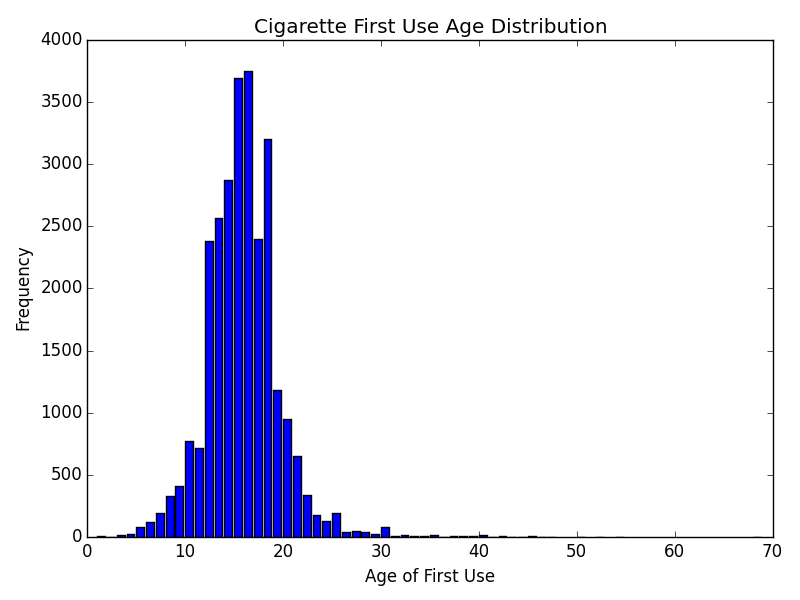
\includegraphics[width=5in]{images/cigAFU}
	\caption{Age of first use with regards to cigarettes}
\end{figure}

\begin{figure}[H]
	\centering
	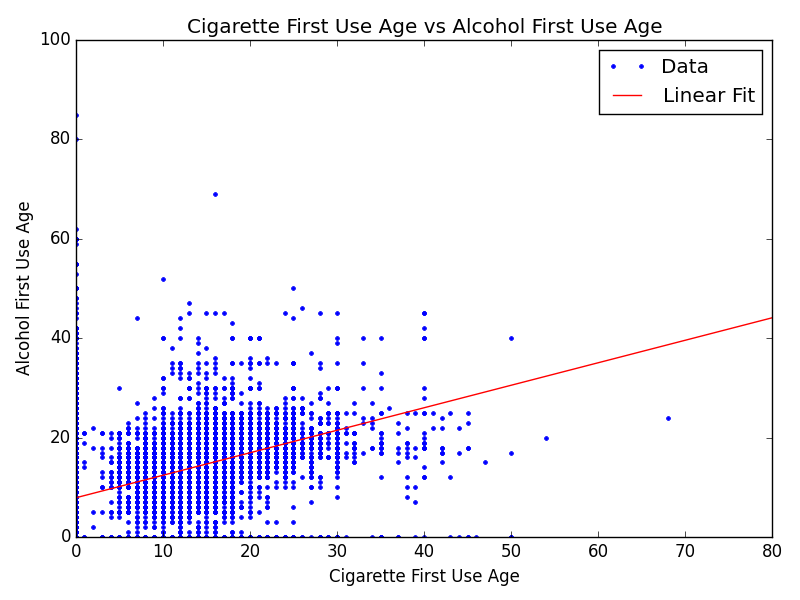
\includegraphics[width=5in]{images/cigVsAlcAFU}
	\caption{A comparison of cigarette and alcohol age of first use}
\end{figure}

Both Figure 4 and 5 are distributed about age 16 in a normal fashion, though each has some interesting spikes which should be noted. For Figure 4 the largest values are seen for ages 14,15,16,17,18, and 21; Figure 5 on the other hand has high values at ages 15,16, and 18. Figure 6 features a large blob of data that appears to be roughly centered at (15,15), but due to the number of data points and the integer values of the data it is difficult to get a good idea of what the relationship between alcohol and cigarette first use age is. In order to provide better insight a linear regression is performed (Ordinary Least Squares slope = 0.452929, intercept = 7.885461, p-value < $10^{-7}$, $r^2$-value = 0.208246, Standard Error = 0.003785) which shows a positive correlation in the data. \\


\subsection*{The Average Number of Drugs}
We can begin to see a relationship between alcohol and cigarette in the survey population, so a natural question that may be posed at this point is how many different drugs the average participant has used? Is it worth investigating relationships between other drugs which have smaller groups of users (and thus less interactions) or do alcohol and tobacco owe their relationship to their relative popularity?

\begin{figure}[H]
	\centering
	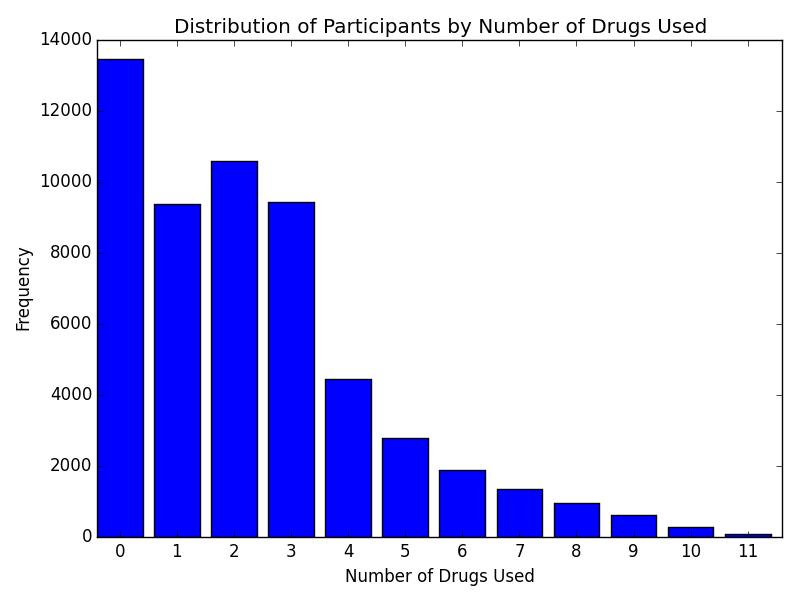
\includegraphics[width=5in]{images/numDrugsUsedDist}
	\caption{The distribution of survey participants based on the number of drug categories they've used}
\end{figure}

The mean number of drugs used by participants of the study is 3.8167. Figure 7 has an interesting shape, it could potentially be a skew distribution with the 0 category as an outliers, or perhaps an exponential decay/power law with 2 and 3 as outliers.\\


\subsection*{The Most Popular Drug}
Another question which is of vital importance is which drug is the most popular? If we wish to reduce the negative effects drugs have on society, then we need to know which drugs have the largest impact. Two measures of popularity have been selected to investigate this, the first is the frequency of participants which use each drug, and the second is the average frequency of use for each drug.

\begin{figure}[H]
	\centering
	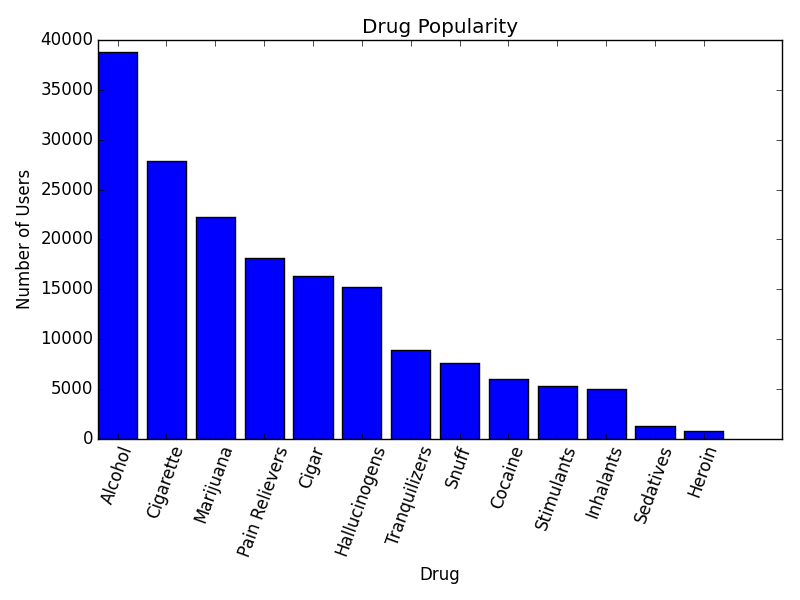
\includegraphics[width=5in]{images/drugPop}
	\caption{Drug popularity by number of users}
\end{figure}

\begin{figure}[H]
	\centering
	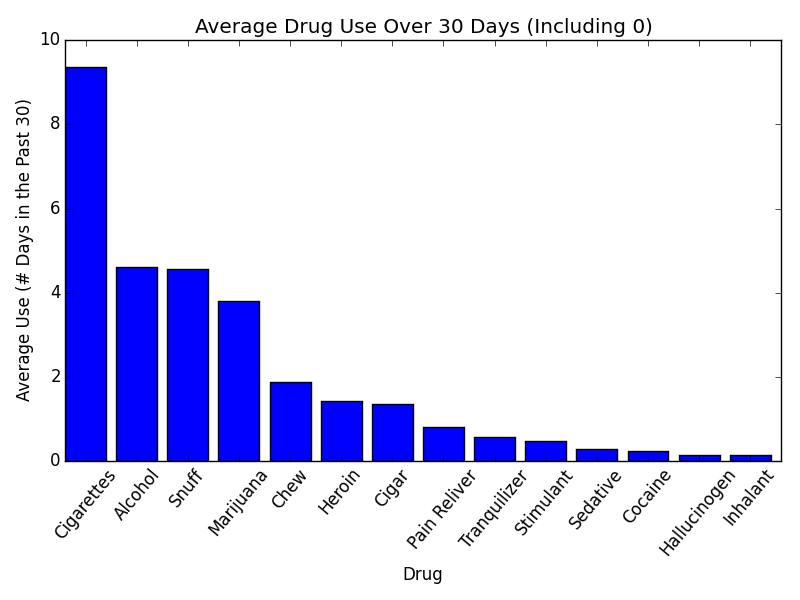
\includegraphics[width=5in]{images/use30With0}
	\caption{Drug popularity by mean frequency of use in the last 30 days}
\end{figure}

\begin{figure}[H]
	\centering
	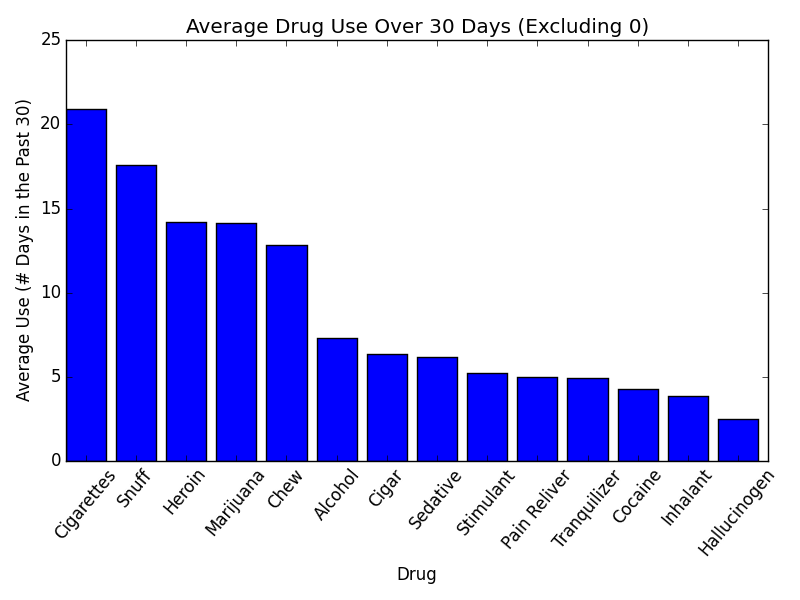
\includegraphics[width=5in]{images/use30}
	\caption{Drug popularity by mean frequency of use in the last 30 days, excludes 0 values}
\end{figure}

The difference between Figures 9 and 10 is the inclusion/exclusion of data points where the survey participant reported using the drug in the past, but not in the last 30 days (ie 0/30). This leads to some interesting differences, the most notable being Heroin and Sedatives which each move up a couple of slots in the ordering.\\

\subsection*{The Most Popular Month}
After looking at what drugs are used, it follows logically that when drugs are used should be investigated as well. In this endeavor the popularity of the months of the year are compared based on the number of participants who reported using a drug for the first time in a given month.

\begin{figure}[H]
	\centering
	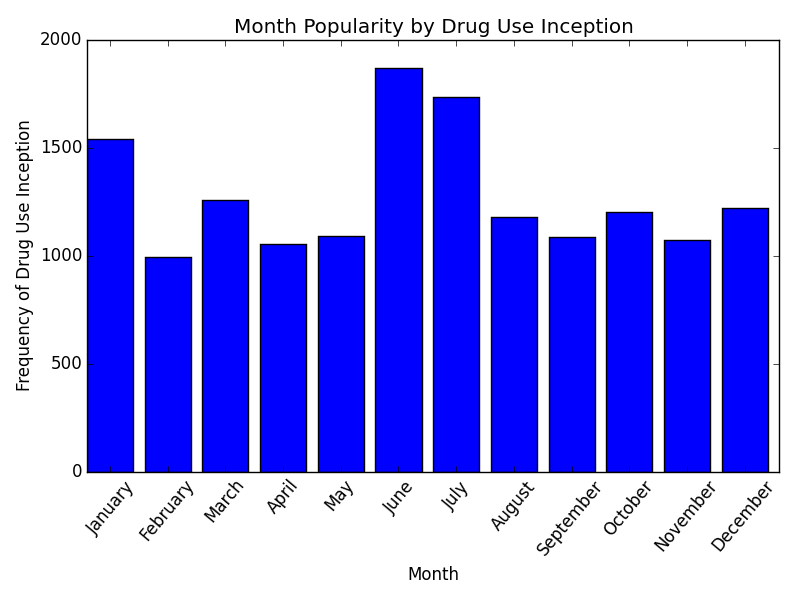
\includegraphics[width=5in]{images/months}
	\caption{Month popularity based on frequency of new drug users}
\end{figure}

It appears that there are abnormally high numbers on new drug users in January, June, and July as well as low number of new drug users in February. In order to confirm that these variations are more than just random chance the Mann-Whitney U test and Kolmogorov-Smirnov test are applied (after the data is normalized) with the null hypothesis being that the data was drawn from a uniform distribution. The two test results agree and both indicate that the data is statistically significantly unique from the uniform distribution (Two Sided MW U-Test: U = 0.00001, p $<$ $10^{-6}$ )(Two Sided KS test: D = 1 , p $<$ $10^{-7}$).\\

\subsection*{Generalized Age of First Use}
In keeping with the theme of when do people use drugs, another graph plotting the distribution of the age of first use of drugs is created. This graph however, will contain data from each drug that was examined in the survey.

\begin{figure}[H]
	\centering
	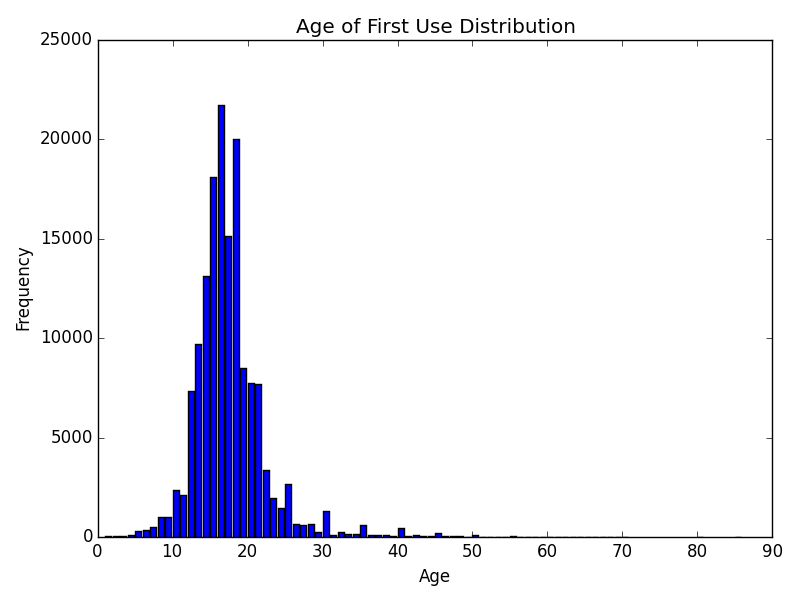
\includegraphics[width=5in]{images/afu}
	\caption{The age of first use plot for all drugs}
\end{figure}

Similar to the age of first use graphs for alcohol and cigarettes, the graph for the conglomerate of drugs has a roughly normal distribution centered at age 16 with the largest frequencies found at ages 15,16, and 18. The spike seen at age 21 for alcohol seems to have smoothed out with the addition of data, and a little more roughness was introduced into the right hand tail of the distribution. The mean of the distribution is 17, the mode is 16, and the median is 16.\\

\subsection*{Age of First Use vs. 30 Day Usage}
Building upon the generalized age of first use plot, we can examine the graph that emerges when you plot the age of first use against the frequency of use in the past 30 days in order to see if using drugs earlier in life influences the amount of drugs you use later in life.

\begin{figure}[H]
	\centering
	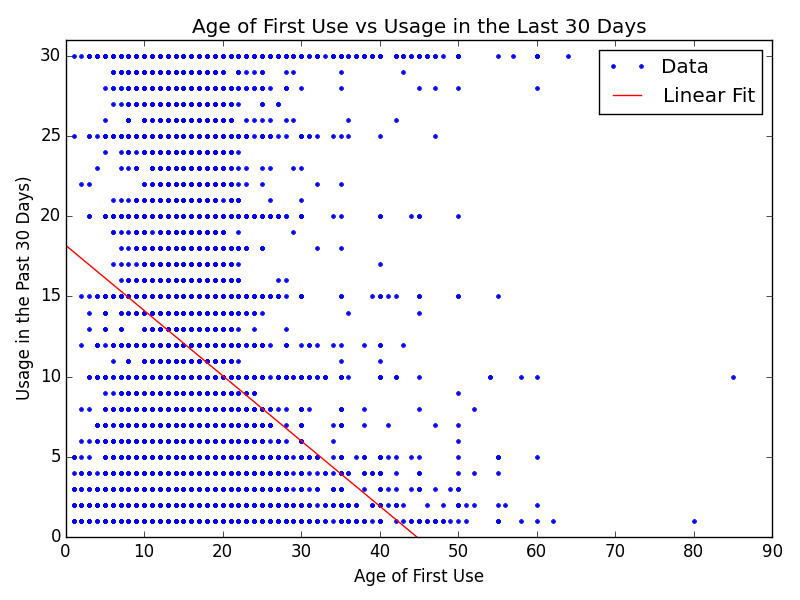
\includegraphics[width=5in]{images/afuVsUse30}
	\caption{The age of first use plot for all drugs}
\end{figure}

Figure 13 has the same problem as Figure 6, the data only has integer values so there is a large amount of overlap between points making it hard to visually inspect the plot. Linear regression is used once again to add insight (Ordinary Least Squares: Slope = -0.406787, Intercept = 18.193414, $r^2$ = 0.022612, P-Value $< 10^{-7}$, Standard Error = 0.011851). \\


\section*{Discussion}
The findings in this report provide multiple insights into the drug usage behavior of the sample population and reveal new questions about the data which require more investigation. Some of the most important findings are that the average person in the survey population has used 3 to 4 drugs (Figure 7), the most popular drugs are alcohol, cigarettes, marijuana, and pain relievers(Figure 8), while the most frequently used drugs are cigarettes, alcohol, snuff, and heroin(Figure 9,10). The most popular months to initiate drug use are January, June, and July, and the most popular age to initiate drug usage is between 15 and 18. Finally, there is a negative correlation between the age when a drug is first used and the current usage frequency.\\

Though many questions were investigated, there are many more left to explore. Statistical methods can be applied to the multiple age of first use distributions to investigate whether they are actually distributed normally. Ordinary least squares provided linear regressions for Figures 6 and 13, and while the p-values were very low in both cases the $r^2$-values were also low. This indicates that a relationship exists but may be non-linear, perhaps curve-fitting or logistic regression will provide better fit lines for these plots. There are also a number of somewhat obvious questions that were not explored in this report including are there any races that are predisposed to use drugs? Is there a correlation between job status or number of hours worked per week and drug use? Does the number of drugs a person has tried correlate with the frequency of drug use? Is drug use correlated with a certain industry or job category?\\

In addition to fleshing out the contents of the report, there is much work that could be done in the realm of finding supporting research. In order to increase the quality of the report and reinforce its findings, it is necessary to find peer-reviewed research which confirms or refutes these findings.

\begin{thebibliography}{1}
	
	\bibitem{DPA} "Drug War Statistics." Drug Policy Alliance. Accessed November 1, 2015. \textcolor{blue}{http://www.drugpolicy.org/drug-war-statistics}.
	
	\bibitem{NIDA}  "Trends \& Statistics." National Institute on Drug Abuse. August 20, 2015. Accessed November 1, 2015. \textcolor{blue}{https://www.drugabuse.gov/related-topics/trends-statistics}. 
	
	\bibitem{USDOH} United States Department of Health and Human Services. Substance Abuse and Mental Health Services Administration. Center for Behavioral Health Statistics and Quality. National Survey on Drug Use and Health, 2012. ICPSR34933-v2. Ann Arbor, MI: Inter-university Consortium for Political and Social Research [distributor], 2014-10-06. \textcolor{blue}{http://doi.org/10.3886/ICPSR34933.v2}.
	
\end{thebibliography}

\end{document}
